\documentclass[ngerman,hyperref={pdfpagelabels=false}]{beamer}

% -----------------------------------------------------------------------------
\graphicspath{{images/}}
\DeclareGraphicsExtensions{.pdf,.png,.jpg}



\usetheme{KIT}

\setbeamercovered{transparent}

\newenvironment<>{KITtestblock}[2][]
{\begin{KITcolblock}<#1>{#2}{KITblack15}{KITblack50}}
{\end{KITcolblock}}

\usepackage[ngerman,english]{babel}
\usepackage[utf8]{inputenc}
\usepackage[TS1,T1]{fontenc}
\usepackage{array}
\usepackage{multicol}
\usepackage[absolute,overlay]{textpos}
\usepackage{graphics}
\usepackage{beamerKITdefs}



\pdfpageattr {/Group << /S /Transparency /I true /CS /DeviceRGB>>}	%required to prevent color shifting withd transparent images


\title{Parallele BVH-Konstruktion auf der GPU}
\subtitle{Daniel Opitz}

\author[Daniel Opitz]{Daniel Opitz}
\institute{Institut für Visualisierung und Datenstrukturen}

\TitleImage[width=\titleimagewd,height=\titleimageht]{images/titel.png}

\KITinstitute{Institut für Visualisierung und Datenstrukturen}
\KITfaculty{Fakultät für Informatik}

% -----------------------------------------------------------------------------

\begin{document}
\setlength\textheight{7cm} %required for correct vertical alignment, if [t] is not used as documentclass parameter


% title frame
\begin{frame}
  \maketitle
\end{frame}


% intro
\section{Introduction}
\begin{frame}
  \frametitle{BVH Konzeptionell}

  \begin{KITcolumns}
  \column{0.49\textwidth}
  \begin{figure}
    \centering
    \includegraphics<1>[width=3cm]{shapes0.pdf}
    \includegraphics<2>[width=3cm]{shapes1.pdf}
    \includegraphics<3>[width=3cm]{shapes2.pdf}
    \includegraphics<4>[width=4cm]{shapes3tree.pdf}
  \end{figure}
  \column{0.49\textwidth}
  \begin{itemize}
    \item<1-> Objekte im Raum
    \item<2-> Bounding Boxen für Objekte
    \item<3-> Konservativ Bounding Boxen zusammenfassen
  \end{itemize}
  \end{KITcolumns}

\end{frame}


\section{Konstruktion}
\begin{frame}
  \frametitle{BVH Konstruktion}

  \heading{Welche Knoten Zusammenfassen?}
  \begin{figure}
    \centering
    \includegraphics<1>[width=6.5cm]{treesplit.png}
  \end{figure}

\end{frame}

\begin{frame}
  \frametitle{BVH Konstruktion}

  \begin{KITcolumns}
  \column{0.49\textwidth}
  \begin{figure}
    \centering
    \includegraphics<1>[width=5cm]{zcurve.png}
    \includegraphics<2>[width=5cm]{mortonsplit.pdf}
  \end{figure}
  \column{0.49\textwidth}
  \begin{itemize}
    \item<1-> Nutze Z-Order-Curve um gute Split-Ebenen zu finden
    \item<1-> Berechne für alle Objekte (Blätter) den zugeörigen Morton-Code
    \item<2-> Sortiere Objekte anhand ihres Morton-Codes
    \item<2-> Finde Split-Ebenen anhand gleicher Präfixe
  \end{itemize}
  \end{KITcolumns}

\end{frame}



\begin{frame}
  \frametitle{BVH - Teilprobleme}
  \framesubtitle{Morton Codes}

  \begin{KITcolumns}
  \column{0.49\textwidth}
  \begin{figure}
    \centering
    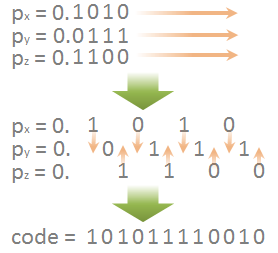
\includegraphics[width=5cm]{bitswizzle.png}
  \end{figure}
  \column{0.49\textwidth}
  \begin{itemize}
    \item Berechne Codes für Schwerpunkte der Blätter
    \item Benötigt Koordinaten in $[0,1]$ $\Rightarrow$ Reduktion zu Wurzel-AABB
    \item Padding der Nachkommateile von x,y und z Komponenten
    \item Verordern zu finalem Morton-Code
  \end{itemize}
  \end{KITcolumns}

\end{frame}



\begin{frame}
  \frametitle{BVH - Teilprobleme}
  \framesubtitle{Radix Sort}

  \begin{KITcolumns}
  \column{0.49\textwidth}
  \begin{figure}
    \centering
    \includegraphics<1>[width=5cm]{sort0.pdf}
    \includegraphics<2>[width=5cm]{sort1.pdf}
    \includegraphics<3>[width=5cm]{sort2.pdf}
    \includegraphics<4>[width=5cm]{sort3.pdf}
  \end{figure}
  \column{0.49\textwidth}
  \begin{itemize}
    \item<1-> Input sind Morton-Codes
    \item<2-> Bestimme ob k-tex bit 0 oder 1 \\ $\texttt{flags}_0[i] = !\texttt{keys}[i]_k$ \\ $\texttt{flags}_1[i] = !\texttt{flags}_0[i]$ 
    \item<3-> Berechen Präfixsumme über \texttt{flags}
    \item<4-> Ordne \texttt{keys} neu
  \end{itemize}
  \end{KITcolumns}

\end{frame}


\begin{frame}[containsverbatim]
  \frametitle{BVH - Teilprobleme}
  \framesubtitle{Radix Sort}

  \begin{itemize}
    \item Für jedes Bit $k$ (LSB $\rightarrow$ MSB)
    \begin{itemize}
      \item Extrahiere $k$-tex Bit aus Morton-Codes
      \item Berechne zwei Präfixsummen (0- und 1-Flags)
      \item Ordne Morton-Codes \emph{und Permutations-Array} neu
    \end{itemize}
  \end{itemize}
  \begin{itemize}
    \item $32 \cdot 2$ Präfixsummen
    \item Reorder-Schritt dominiert Laufzeit
    \item Breakeven (Laptop) bei $\sim$15K Elementen
  \end{itemize}

\end{frame}


\begin{frame}
  \frametitle{BVH Konstruktion}
  \framesubtitle{Hierarchie erstellen}

  \begin{KITcolumns}
  \column{0.49\textwidth}
  \begin{figure}
    \centering
    \includegraphics<1>[width=5cm]{treesplit.png}
  \end{figure}
  \column{0.49\textwidth}
  \begin{itemize}
    \item<1-> Innere Knoten repräsentiert als Index-Range
    \item<1-> Kindknoten unterteilen Index-Range des Elternknoten an genau einer Stelle
    \item<1-> Hierarchisches Vorgehen von Wurzel richtung Blätter möglich
    \item<1-> \textbf{Aber}: Schlechte Auslastung der GPU
  \end{itemize}
  \end{KITcolumns}

\end{frame}


\begin{frame}
  \frametitle{BVH Konstruktion}
  \framesubtitle{Hierarchie erstellen}

  \begin{KITcolumns}
  \column{0.49\textwidth}
  \begin{figure}
    \centering
    \includegraphics<1>[width=5cm]{nodes.png}
  \end{figure}
  \column{0.49\textwidth}
  \begin{itemize}
    \item<1-> \textbf{Besser}: Finde für jeden Knoten zu erst seine Index-Range
      \begin{itemize}
        \item Knoten-Startposition \\+ zwei binäre Suchen
      \end{itemize}
    \item<1-> Finde Split-Index mit binärer Suche
    \item<1-> Mehr arbeit in jedem Thread, aber alle inneren Knoten parallel
  \end{itemize}
  \end{KITcolumns}

\end{frame}


\begin{frame}
  \frametitle{Demo}

\end{frame}






\end{document}

